\section{DETAILS OF Maat}
In this section, we first outline the design rationale of Maat (\S III-A). Then the overall framework and workflow of Maat are described in detail (\S III-B \& \S III-C). Finally, the mechanism for Maat to fully maintain PCC is introduced (\S III-D). The main symbols used in Maat are shown in Table I.

\begin{table}[hbp]
	\centering
	\caption{Symbols frequently used in Maat.}
	\label{table1}
	\begin{tabular}{|m{1cm}<{\centering}|m{7cm}|}
		\hline
		Symbol & Description \\ \hline
		$\Delta$ & Flow size threshold used to identify load imbalance among servers \\ \hline
		\emph{$S_i$} & The \emph{$i^{th}$} server (DIP) \\ \hline
		\emph{$T[\emph{$S_i$}]$} & The total flow size of the \emph{$i^{th}$} server \\ \hline
		\emph{$B[\emph{$S_i$}]$} & The backup server of the \emph{$i^{th}$} server \\ \hline
		\emph{$F[\emph{$S_i$}]$} & Boolean value used to identify whether the \emph{$i^{th}$} server is acting as a backup server \\ \hline
	\end{tabular}
\end{table}

\subsection{Rationale of Maat} 
Maat is designed with two dimensions in mind: 1) Unlike existing L4 LBs that only use hash functions to select servers, Maat selects the less loaded server from two choices: one selected by hash and one selected randomly, which improves fairness. 2) Maat divides the incoming traffic into two categories, one is sent to hash-selected servers, and the other is sent to randomly selected servers. This approach helps resolve potential PCC violations with negligible memory overhead. By utilizing these two dimensions, Maat successfully meets both L4 LB requirements—maintaining PCC and improving fairness—without requiring modifications to the existing network infrastructure.


\begin{figure}[t]
	\setlength{\abovecaptionskip}{0pt}
	\setlength{\belowcaptionskip}{-10pt}
	\centering
	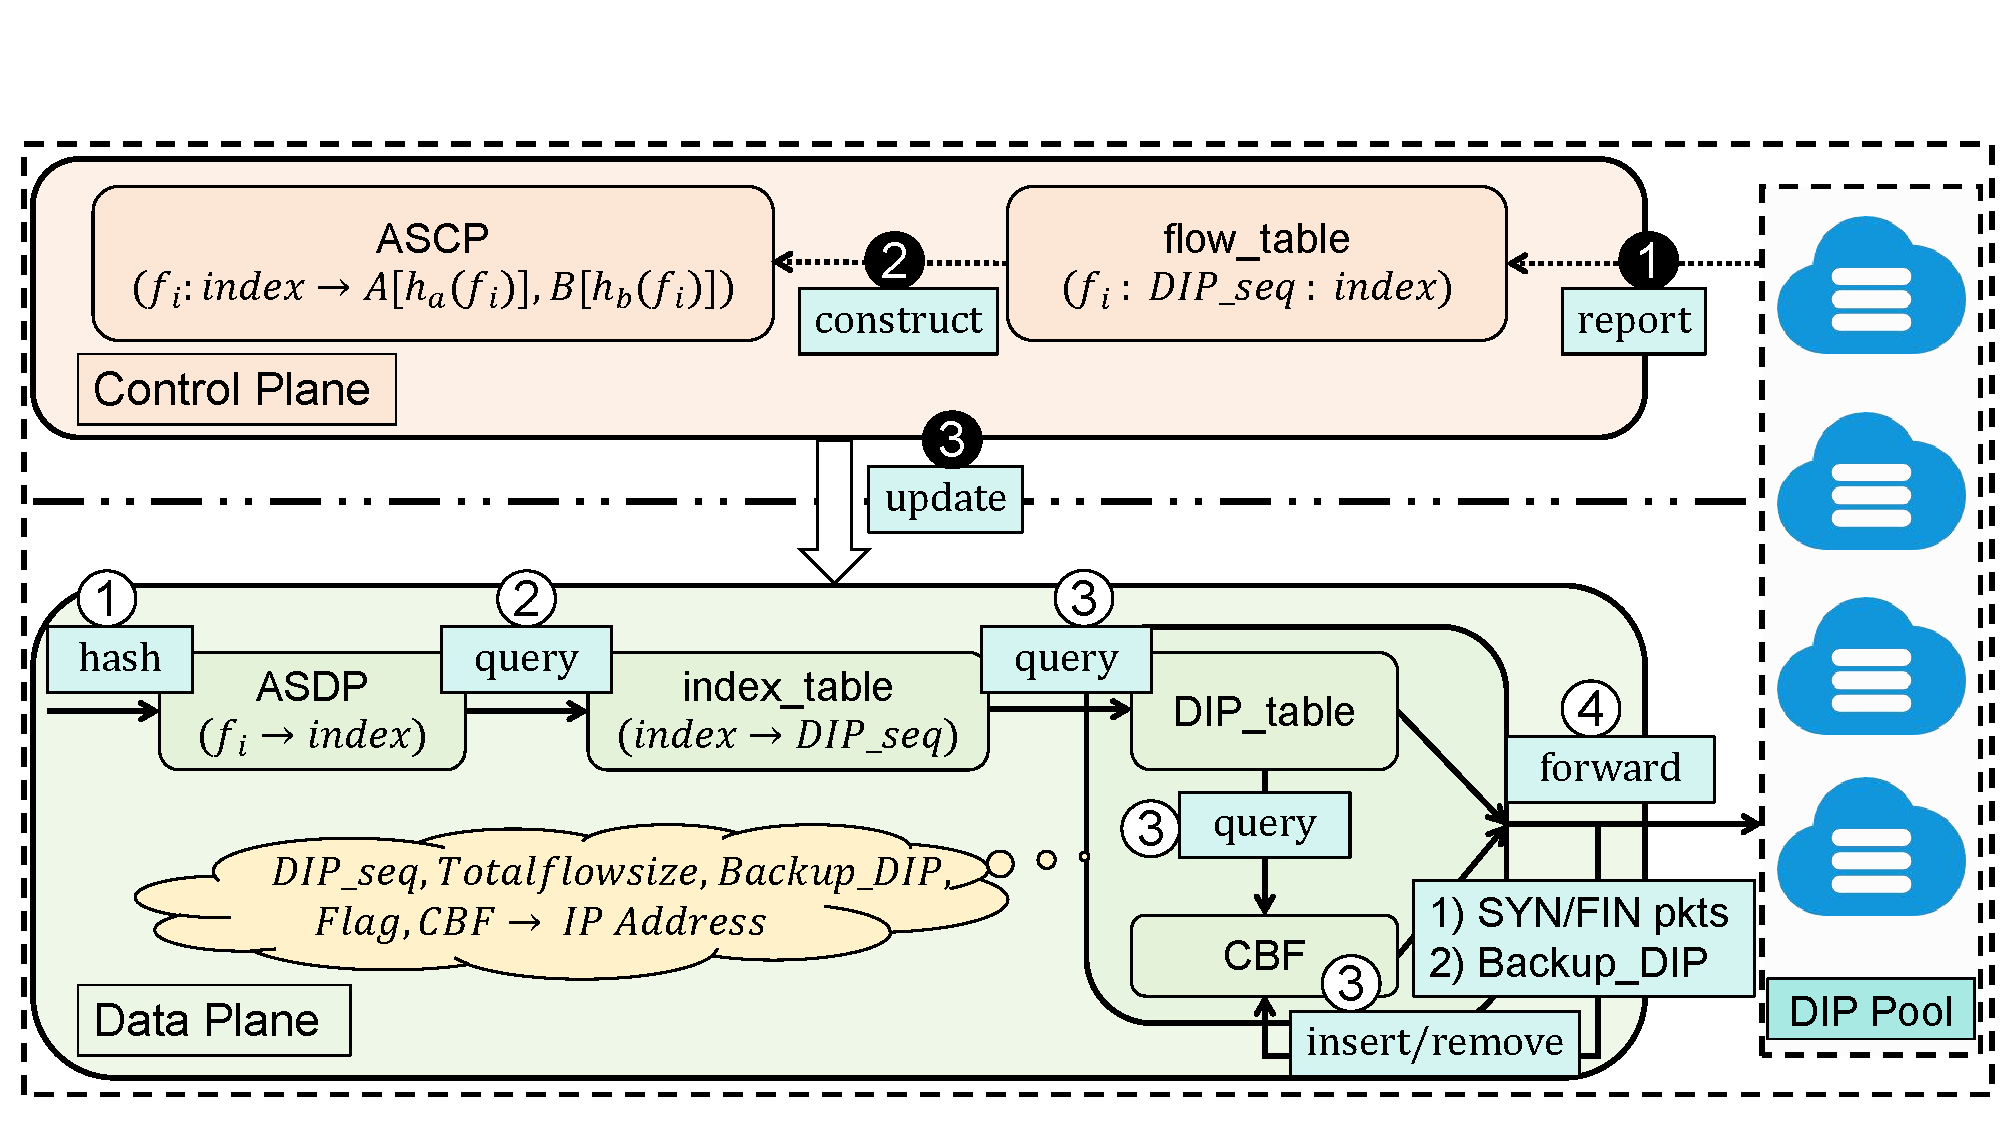
\includegraphics[width=1\linewidth]{figure/framework.pdf}
	\caption{Framework of Maat.}
	\label{5}
\end{figure}

\subsection{Frameworks of Maat}
Fig. \ref{5} shows the framework and workflow of Maat. In the data plane, we propose a scheduling method called the power of one random choice for enhancing fairness. Meanwhile, we also integrate Othello hashing and counting Bloom filters into Maat to mitigate potential PCC violations. In the control plane, our main concern is to update the data plane in real-time in response to changes in the DIP pool.

Maat is mainly composed of six major components:

(1) ASDP (Array Sets on Data Plane) is implemented by Othello hashing structure \cite{yu2018memory}, which consists of two arrays, \emph{A} and \emph{B}. Its main function is to query the corresponding \emph{index} for each flow. For example, with \emph{$f_{\text{3}}$} in Fig. \ref{4}, we first use \emph{$h_a$} and \emph{$h_b$} to calculate the hash values of \emph{$f_{\text{3}}$}, then use XOR to calculate \emph{A}[\emph{$h_a(f_{\text{3}})$}] (\emph{$a_4$}=$10_2$) and \emph{B}[\emph{$h_b(f_{\text{3}})$}] (\emph{$b_3$}=$00_2$). Finally, we can get that the \emph{index} corresponding to \emph{$f_{\text{3}}$} is 2.

(2) index\_table establishes a mapping relationship between \emph{index} and \emph{DIP_seq}. This is a many-to-one mapping \cite{olteanu2018stateless}, where multiple different \emph{index} values may map to the same \emph{DIP_seq}. \emph{DIP_seq} has a static mapping relationship with the IP address of the DIP. The \emph{index} is introduced to reduce memory consumption. Because the server's IP address is 32 bits, while the \emph{index} is usually much smaller, such as 8 bits \cite{shi2020concury}. Additionally, the number of \emph{index} mapped by each \emph{DIP_seq} can also be used to illustrate the weight (load status) of the server.

(3) DIP\_table is the core component of Maat and is responsible for forwarding packets to the appropriate server. It describes the status information of all servers (DIPs) running the same service. As shown in Fig. \ref{7}, it includes the following five fields: 1) \emph{DIP_seq}: A one-to-one mapping with the DIP's actual IP address. 2) \emph{IP Address}: The actual IP address of the DIP, is used to modify the destination IP address in the packet header. 3) \emph{Totalflowsize (T)}: Maat directly counts the number of packets of all flows processed on each server, rather than distinguishing which flows are large flows and which flows are small flows like the previous solution \cite{guo2022libra}. This method can more accurately reflect the impact of traffic on the server load (see Fig. \ref{9}). 4) \emph{Backup_DIP (B)}: This field is used to record the backup server of \emph{$S_i$}, The backup server \emph{$B[\emph{$S_i$}]$} is randomly selected to ensure load fairness among servers. As shown in Fig. \ref{7.2}, the backup server of \emph{$S_1$} is \emph{$S_2$}. 5) \emph{Flag (F)}: A boolean field, defaulting to false. When \emph{$S_1$} is selected as the backup for \emph{$S_2$}, the \emph{Flag} of \emph{$S_1$} is set to true to prevent other servers (e.g., \emph{$S_3$}) from selecting \emph{$S_1$} as their backup server. This field is introduced to achieve better load balancing between servers (see \S III-C1 for details).

(4) counting Bloom filter (CBF) is one of the variants of Bloom filter (BF) \cite{geravand2013bloom}. BF is a highly space-saving probabilistic data structure that enables efficient insertion and querying. CBF supports deletion operations based on BF, making CBF more suitable for dynamically changing data sets such as network traffic. CBF is primarily used to avoid potential PCC violations.

(5) flow\_table maintains the mapping relationship between \emph{$f_{\text{i}}$} and the server (DIP) on the control plane, recording the latest flows processed by the servers. It works by using a lightweight application-layer program to track the flow status of each server, which has been deployed to LB \cite{gandhi2014duet} in current data centers without changing the network stack. Whenever the flow status on the servers changes (e.g., flow arrival or termination), the servers report to LB, and then LB uses these reports to update flow\_table.

(6) ASCP (Array Sets on Control Plane) is also implemented by the Othello hashing structure but serves a different role than ASDP. Maat uses the latest mapping relationship in flow\_table to construct ASCP. Whenever the DIP pool updates, ASCP can quickly (microsecond level) update the data plane \cite{shi2020concury} to ensure that PCC violations not occur in Maat when the DIP pool changes, except in the case of server failure.

\subsection{Workflow of Maat}
(1) Data plane: The data plane of Maat is the key to achieving the two requirements (fairness \& PCC). For all incoming traffic, the LB selects an appropriate server among those running the corresponding service, rewrites the destination IP field in the packet header, and forwards it to the selected server. Maat's processing of packets is divided into two situations \cite{shi2020concury}: 1) Stateless packets. The flow to which the packet belongs has not selected any server. For example, for the first packet of each flow, LB needs to select a server for forwarding according to the pre-specified scheduling method; 2) Stateful packets. Unlike stateless packets, the flow to which the packet belongs has been processed. The LB needs to forward the packet to a specific server to ensure that all packets of the same connection are forwarded to the same server (PCC). Next, we describe in detail how the data plane handles these two types of packets.

1) Stateless packets: When Maat receives a stateless packet, such as the first packet (SYN=1) of a certain TCP flow (\emph{$f_i$}). We first query the \emph{index} corresponding to the flow in the ASDP (\ding{172}). Next, we find the \emph{DIP_seq} corresponding to the \emph{index} in the index\_table (\ding{173}), and finally, we find the hash-selected server in DIP\_table (assume {\emph{$S_1$}). We then process the stateless packets based on the power of one random choice (\ding{174}). We handle the following two situations according to Algorithm 1.
	
\begin{figure}[t]
	\setlength{\abovecaptionskip}{0pt}
	\setlength{\belowcaptionskip}{-10pt}
	\centering
	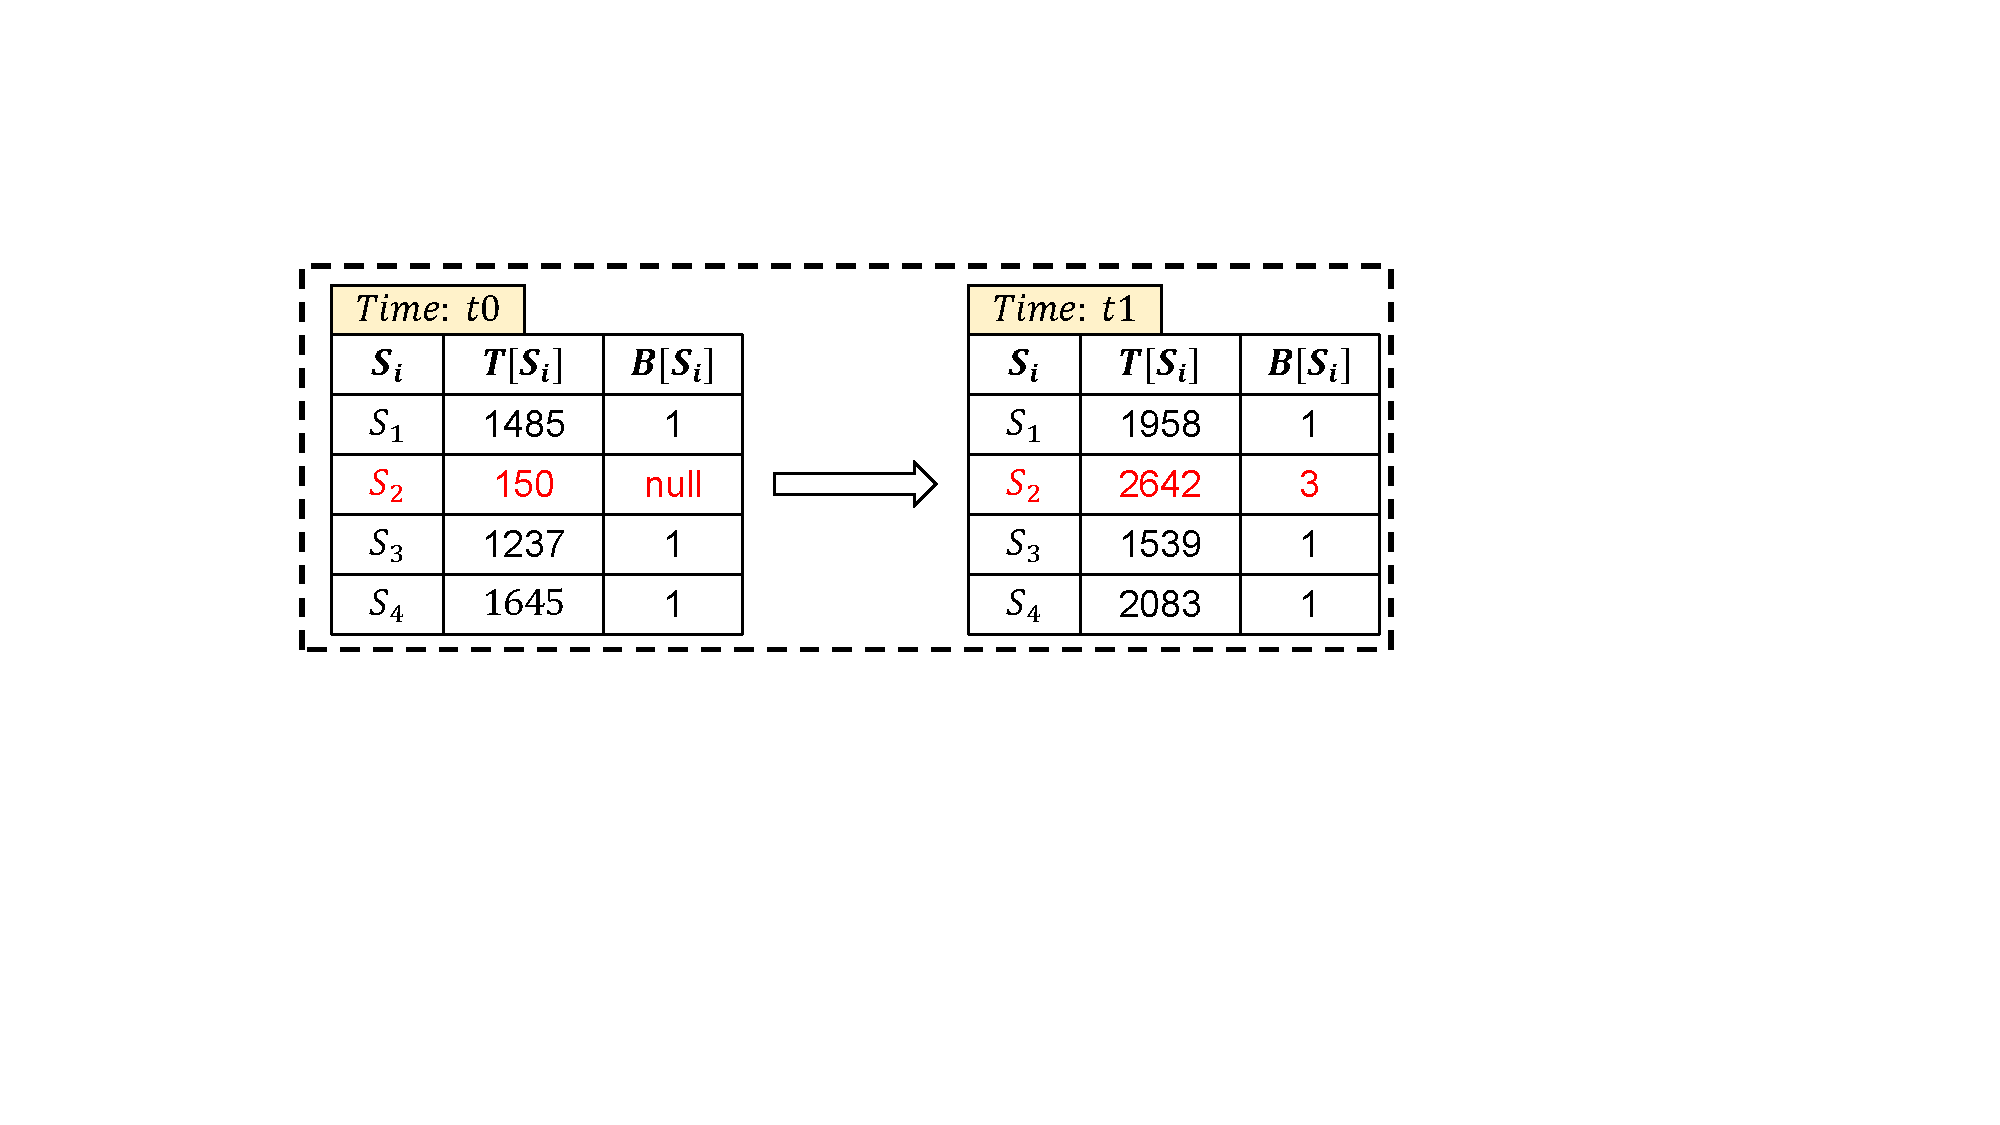
\includegraphics[width=1\linewidth]{figure/flag.pdf}
	\caption{Reason for introducing \emph{Flag} field in DIP_table ($\textbf{t1} > \textbf{t0}$, $\Delta = 1000 (packets)$).}
	\label{6}
\end{figure}

\textbf{Case 1.} \emph{B}[\emph{$S_1$}] is \emph{null}. In this case, \emph{$S_1$} may have a load imbalance with other servers, so we randomly select a server (assume \emph{$S_2$}). If $\emph{T}[\emph{$S_1$}] - \emph{T}[\emph{$S_2$}] \geq \Delta$ and $\emph{F}[\emph{$S_2$}] = \emph{false}$, where $\Delta$ is a predefined threshold indicating whether the flow should be forwarded to the backup server (Lines 1-8). The former condition shows that the load of \emph{$S_1$} is much greater than the load of \emph{$S_2$}, there is a load imbalance between \emph{$S_1$} and \emph{$S_2$}, and the latter indicates \emph{$S_2$} can serve as the backup server of \emph{$S_1$}. Thus, we set \emph{F}[\emph{$S_2$}] is \emph{true} and \emph{B}[\emph{$S_1$}] is \emph{$S_2$}, insert the flow into CBF (\ding{174}) to prevent PCC violation (see \S III-D for details), and finally forward the flow to \emph{$ S_2$} (\ding{175}). 

If either of the above two conditions is not met, i.e., $\emph{T}[\emph{$S_1$}] - \emph{T}[\emph{$S_2$}] \leq \Delta$ or $\emph{F}[\emph{$S_2$}] = \emph{true}$, it indicates that \emph{$S_1$} and \emph{$S_2$} may load balance or the load of \emph{$S_1$} is smaller than \emph{$S_2$}, or \emph{$S_2$} is already a backup server for other servers (Lines 9-11). In these cases, we should forward the packet to \emph{$S_1$} (\ding{175}) to achieve better fairness. We introduce the \emph{Flag} field in DIP_table to avoid scenarios like Fig. \ref{6}, where at \textbf{t0}, the load of \emph{$S_2$} is significantly lower than \emph{$S_1$}, \emph{$S_3$} and \emph{$S_4$}. Without the \emph{Flag} field, \emph{$S_2$} could be selected as a backup server by the other three servers. \emph{$S_2$} may handle too much load and become unbalanced with other servers at \textbf{t1}. This is caused by \emph{$S_2$} being selected as a backup server by multiple servers. In our tests, not introducing \emph{Flag} field lead to a 28.12\% decrease in fairness, and as the workload increases, this imbalance becomes more and more serious, especially in the case of long-tail distributions.

\textbf{Case 2.} \emph{B}[\emph{$S_1$}] is not \emph{null}. There may be a load imbalance between \emph{$S_1$} and \emph{B}[\emph{$S_1$}]. We compare the loads of \emph{$S_1$} and \emph{B}[\emph{$S_1$}]. If \emph{T}[\emph{$S_1$}] is much larger than \emph{T}[\emph{B}[\emph{$S_1$}]], and the difference exceeds $\Delta$, which means there is a serious load imbalance between \emph{$S_1$} and \emph{B}[\emph{$S_1$}] (Lines 12-16). Maat insert this flow into CBF (\ding{174}), forwarding the packet to \emph{B}[\emph{$S_1$}] (\ding{175}). On the contrary, it means that there is load balancing between \emph{$S_1$} and \emph{B}[\emph{$S_1$}], and the stateless packet is still forwarded to {\emph{$S_1$}} (Lines 17-19).

2) Stateful packets: When Maat receives a stateful packet (belonging to \emph{$f_i$}), our goal is no longer to select the appropriate server based on the scheduling method, but to ensure that the connection where the packet is located not be broken. Similarly, we find the correct \emph{index} and \emph{DIP_seq} in ASDP (\ding{172}) and index_table (\ding{173}) respectively. We can find the server selected by the hash function (assume \emph{$S_1$}). Next, we use the power of one random choice in the DIP_table  (\ding{174}) to handle the following two situations:

\textbf{Case 1.} \emph{B}[\emph{$S_1$}] is \emph{null} (Lines 20-22). In this case, \emph{$S_1$} has not selected any server as a backup server. We only need to forward the packet to \emph{$S_1$} (\ding{175}), which ensures that all packets belonging to the same connection are forwarded to the same server, that is, no PCC violation occurs.


\textbf{Case 2.} \emph{B}[\emph{$S_1$}] is not \emph{null} (Lines 23-29). To maintain PCC, we need to confirm that the currently processed flow is forwarded to \emph{$S_1$} or \emph{B}[\emph{$S_1$}]. Here, we use CBF (see \S III-D for details). If the flow record is found in CBF (\ding{174}), the flow is forwarded to \emph{B}[\emph{$S_1$}] (\ding{175}). If there is no related record, the flow is forwarded to \emph{$S_1$} (\ding{175}).

\begin{algorithm}[t]
	\caption{power of one random choice}
	\label{alg:example}
	\SetKwInOut{Input}{Input}
	\SetKwInOut{Output}{Output}
	
	\Input{A stateless/stateful packet of flow $f_i$, \\ 
		Hash selected server: \emph{$S_1$}, \\
		Threshold: $\Delta$}
	\Output{The server to handle the flow $f_i$}
	
	\tcp{A stateless packet of flow $f_i$}
	\If{ \emph{B}{$[\emph{$S_1$}]$} is null} {
		Random select server (\emph{$S_2$}); \\
		\If{ $\emph{T}[\emph{$S_1$}] - \emph{T}[\emph{$S_2$}] \geq \Delta$ \textbf{and} $\emph{F}[\emph{$S_2$}] = false$} {
			\emph{B}[\emph{$S_1$}] = \emph{$S_2$}; \\
			\emph{F}[\emph{$S_2$}] = \emph{true};  \\ \emph{T}[\emph{$S_2$}]++; \\
			\emph{CBF.insert($f_i$)}; \\
			\textbf{return} \emph{$S_2$};
		} \Else{
			\emph{T}[\emph{$S_1$}]++; \\
			\textbf{return} \emph{$S_1$};
		}
	} \Else{
		\If{$\emph{T}[\emph{$S_1$}] - \emph{T}[\emph{B$[\emph{$S_1$}]$}] \geq \Delta $} {
			\emph{T}[\emph{B$[\emph{$S_1$}]$}]++; \\
			\emph{CBF.insert($f_i$)}; \\
			\textbf{return} \emph{B}[\emph{$S_1$}]; \\
		} \Else{
			\emph{T}[\emph{$S_1$}]++; \\
			\textbf{return} \emph{$S_1$};
		}
	}
	
	\tcp{A stateful packet of flow $f_i$}
	\If{\textbf{B[\emph{$S_1$}]} is null} {
		\emph{$\emph{T}[\emph{$S_1$}]$}++; \\
		\textbf{return} \emph{$S_1$};
	} \Else{
		\If{${\emph{CBF.query($f_i$)}} = true$} {        \emph{T}[\emph{B$[\emph{$S_1$}]$}]++; \\
			\textbf{return} \emph{B}[\emph{$S_1$}];
		} \Else {
			\emph{T}[\emph{$S_1$}]++; \\
			\textbf{return} \emph{$S_1$};
		}
	}
\end{algorithm}

As shown in Fig. \ref{7.1}, the first packet of $f_1$ is hashed to select \emph{$S_2$}. Then, by using the power of one random choice, Maat randomly selects \emph{$S_1$}, and finally, forwards the first packet of $f_1$ to \emph{$S_2$} according to the judgment condition. Other situations can also be processed according to Algorithm 1, and the incoming packets are forwarded to the appropriate server to meet the requirements of L4 LB for fairness and PCC.

As seen from the workflow of the Maat data plane, the power of one random choice combines the advantages of the hash algorithm and the power of two choices cleverly. Initially, hash selection plays a key role in significantly reducing PCC violations. At the same time, through one random choice, the utilization of all server resources is improved, thereby greatly enhancing load fairness among servers. Subsequent experiments demonstrate that this algorithm not only effectively preserves PCC but also enhances fairness.

(2) Control plane: The main task of the control plane is to promptly update the latest mapping relationship between flow and DIP to the data plane when the network changes. This function is similar to the control plane in most previous works \cite{miao2017silkroad, eisenbud2016maglev, zhang2021loom}.  The control plane interacts with the lightweight programs running on each server \cite{gandhi2014duet}. Whenever the control plane receives a report from the server, flow_table is updated (\ding{182}). Afterward, Maat(\ding{183}) constructs the latest ASCP through addition/deletion operations. The time complexity of related operations is \emph{$O(1)$} \cite{yu2018memory}. Whenever the DIP pool changes, the control plane can use ASCP to construct the latest ASDP for the data plane, clears the CBF, index\_table and DIP\_table is updated to forward traffic to the new DIP pool, where \emph{T},\emph{B} and \emph{F} of DIP_table are reset (\ding{184}).


\subsection{Keep PCC}
Related work \cite{shi2020concury} has mentioned that the Othello hashing structure can guarantee PCC regardless of network changes (e.g., DIP pool updates). However, when Maat applies this structure to hash selection in the power of one random choice mechanism, PCC violations may occur. In Fig. \ref{7.1}, the hash selection of \emph{$f_1$} is \emph{$S_2$}, but the random selection is \emph{$S_1$}. It is observed that there is a load balance between \emph{$S_2$} and \emph{$S_1$}, therefore, the packet is forwarded to \emph{$S_2$}. In Fig. \ref{7.2}, the hash selection of \emph{$f_2$} is \emph{$S_2$}, and the random selection is \emph{$S_3$}. However, there is a load imbalance between \emph{$S_2$} and \emph{$S_3$}, so Maat forwards \emph{$f_2$} to \emph{$S_3$} to alleviate the load imbalance. Although the hash selections for \emph{$f_1$} and \emph{$f_2$} are both \emph{$S_2$}, the final server selection is different: \emph{$f_1$} is forwarded to \emph {$ S_2$}, while \emph{$f_2$} is forwarded to \emph{$S_3$}. Each flow may have two choices: 1) a hash-selected server; or 2) a randomly selected server. If the selection of each flow cannot be distinguished, a PCC violation is likely to occur.

The basic approach involves utilizing an additional table to store the relationship between the connection and the backup server. However, to minimize memory usage, we can elegantly transform this key-value store challenge into a more simplified membership set problem \cite{gandhi2014duet}. For this problem, we adopt the counting Bloom filter (CBF) as a solution, CBF is a space-efficient random data structure that can efficiently determine whether an element belongs to a set. Specifically, when a flow is forwarded to the backup server, for SYN packets, we insert this flow into CBF, and for FIN packets, we remove this flow from CBF, and for other packets, we query CBF to confirm whether to forward them to the backup server. In Fig. \ref{7.3}, considering \emph{$f_1$} and \emph{$f_2$}, \emph{$f_2$} needs to be inserted into CBF. Then, for subsequent packets from \emph{$f_1$} and \emph{$f_2$}, a simple query in the CBF can determine whether to forward the packet to \emph{$S_2$} or \emph{$S_3$}, thus helping us avoid potential PCC violations. Furthermore, whenever the control plane updates the data plane, the data plane can maintain the latest mapping relationship, so we only need to clear CBF when updating the data plane. With the integration of CBF, Maat effectively addresses potential PCC violations with minimal memory overhead, even under heavy load.

    \begin{figure}[t]
	\setlength{\abovecaptionskip}{0pt}
	\setlength{\belowcaptionskip}{-10pt}
	\centering  %图片全局居中
	\subfigure[$f_1$ forward to \emph{$S_2$} (IP Address: 192.168.1.2).]{
		\label{7.1}
		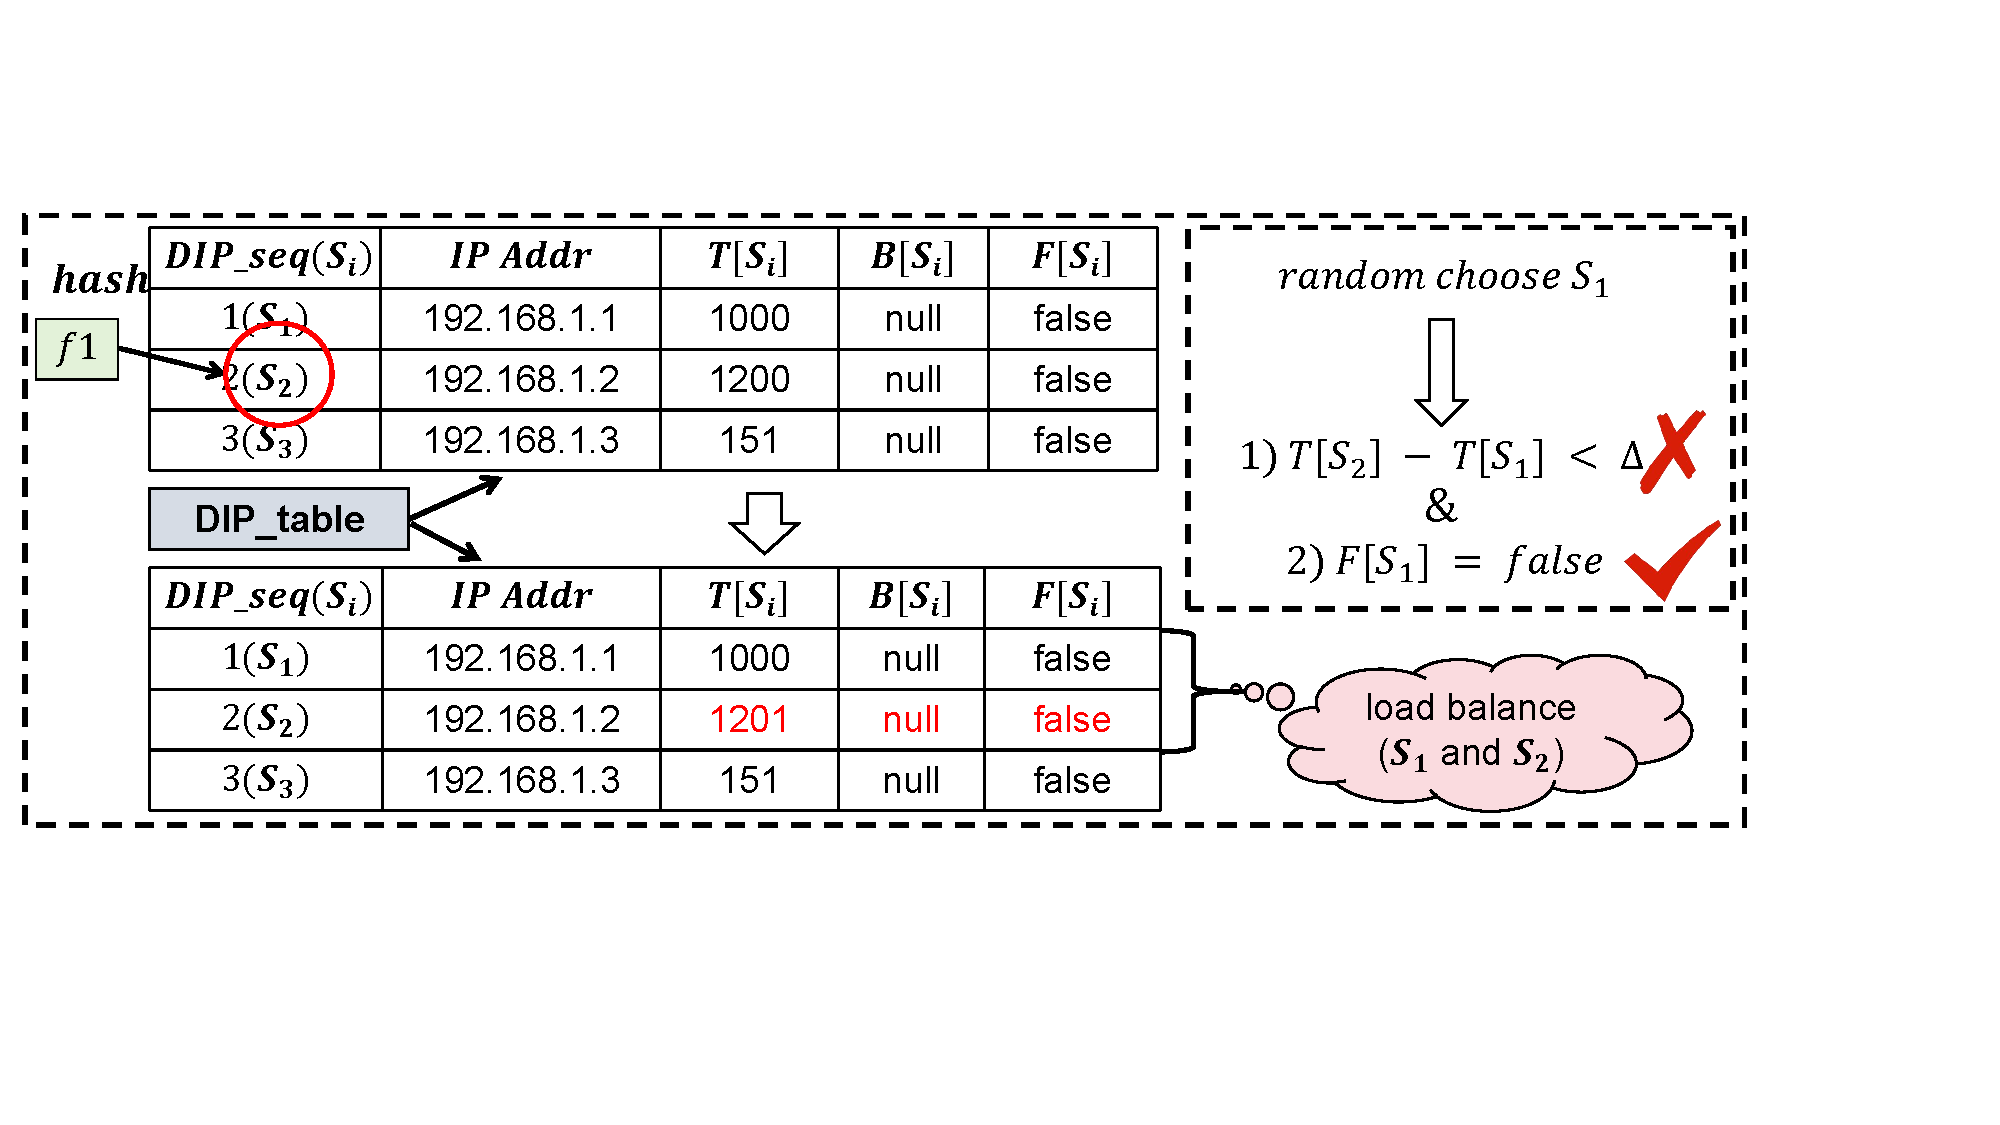
\includegraphics[width=1\linewidth]{figure/keeppcc1.pdf}}\\
	\subfigure[$f_2$ forward to \emph{$S_3$} (IP Address: 192.168.1.3).]{
		\label{7.2}
		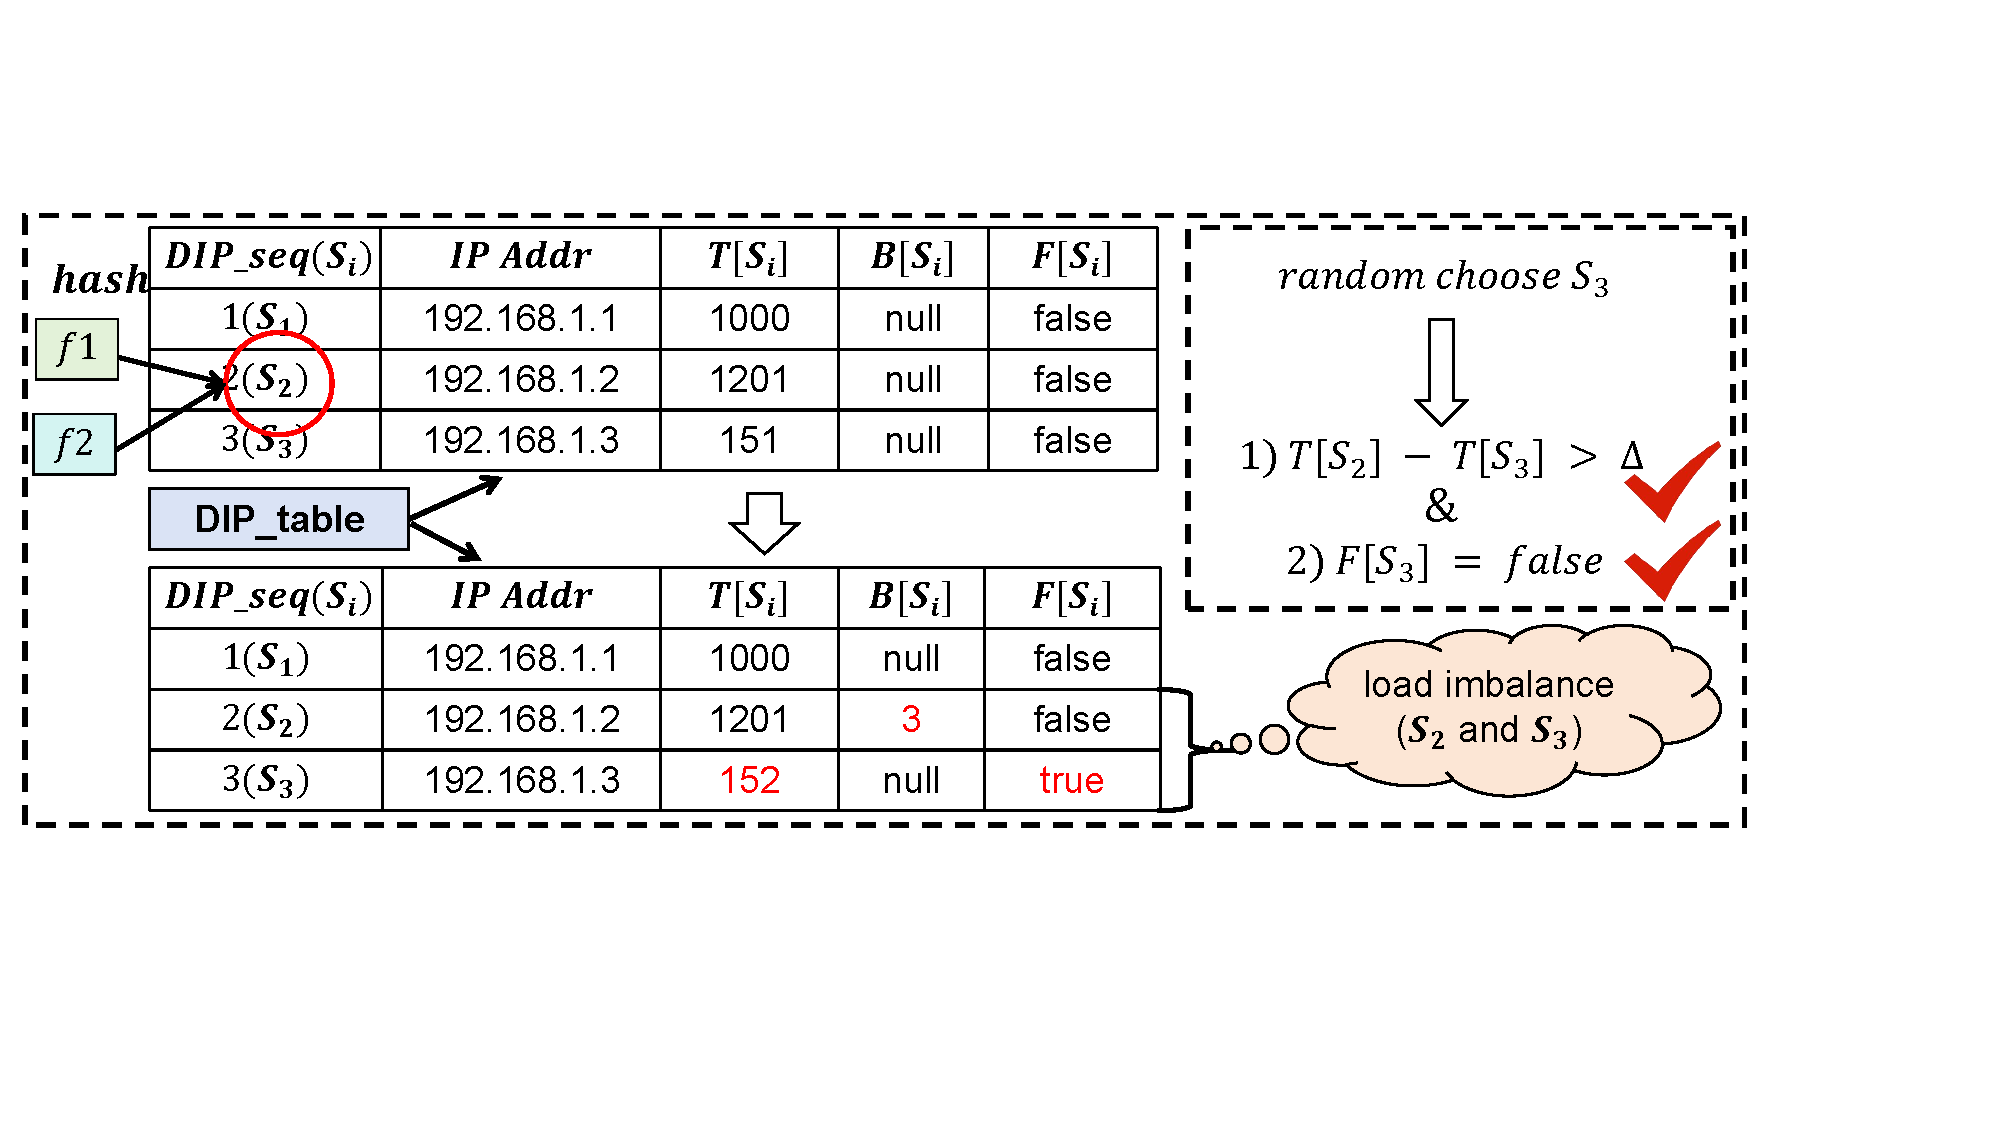
\includegraphics[width=1\linewidth]{figure/keeppcc2.pdf}}
	\subfigure[$f_2$ insert \textbf{CBF}.]{
		\label{7.3}
		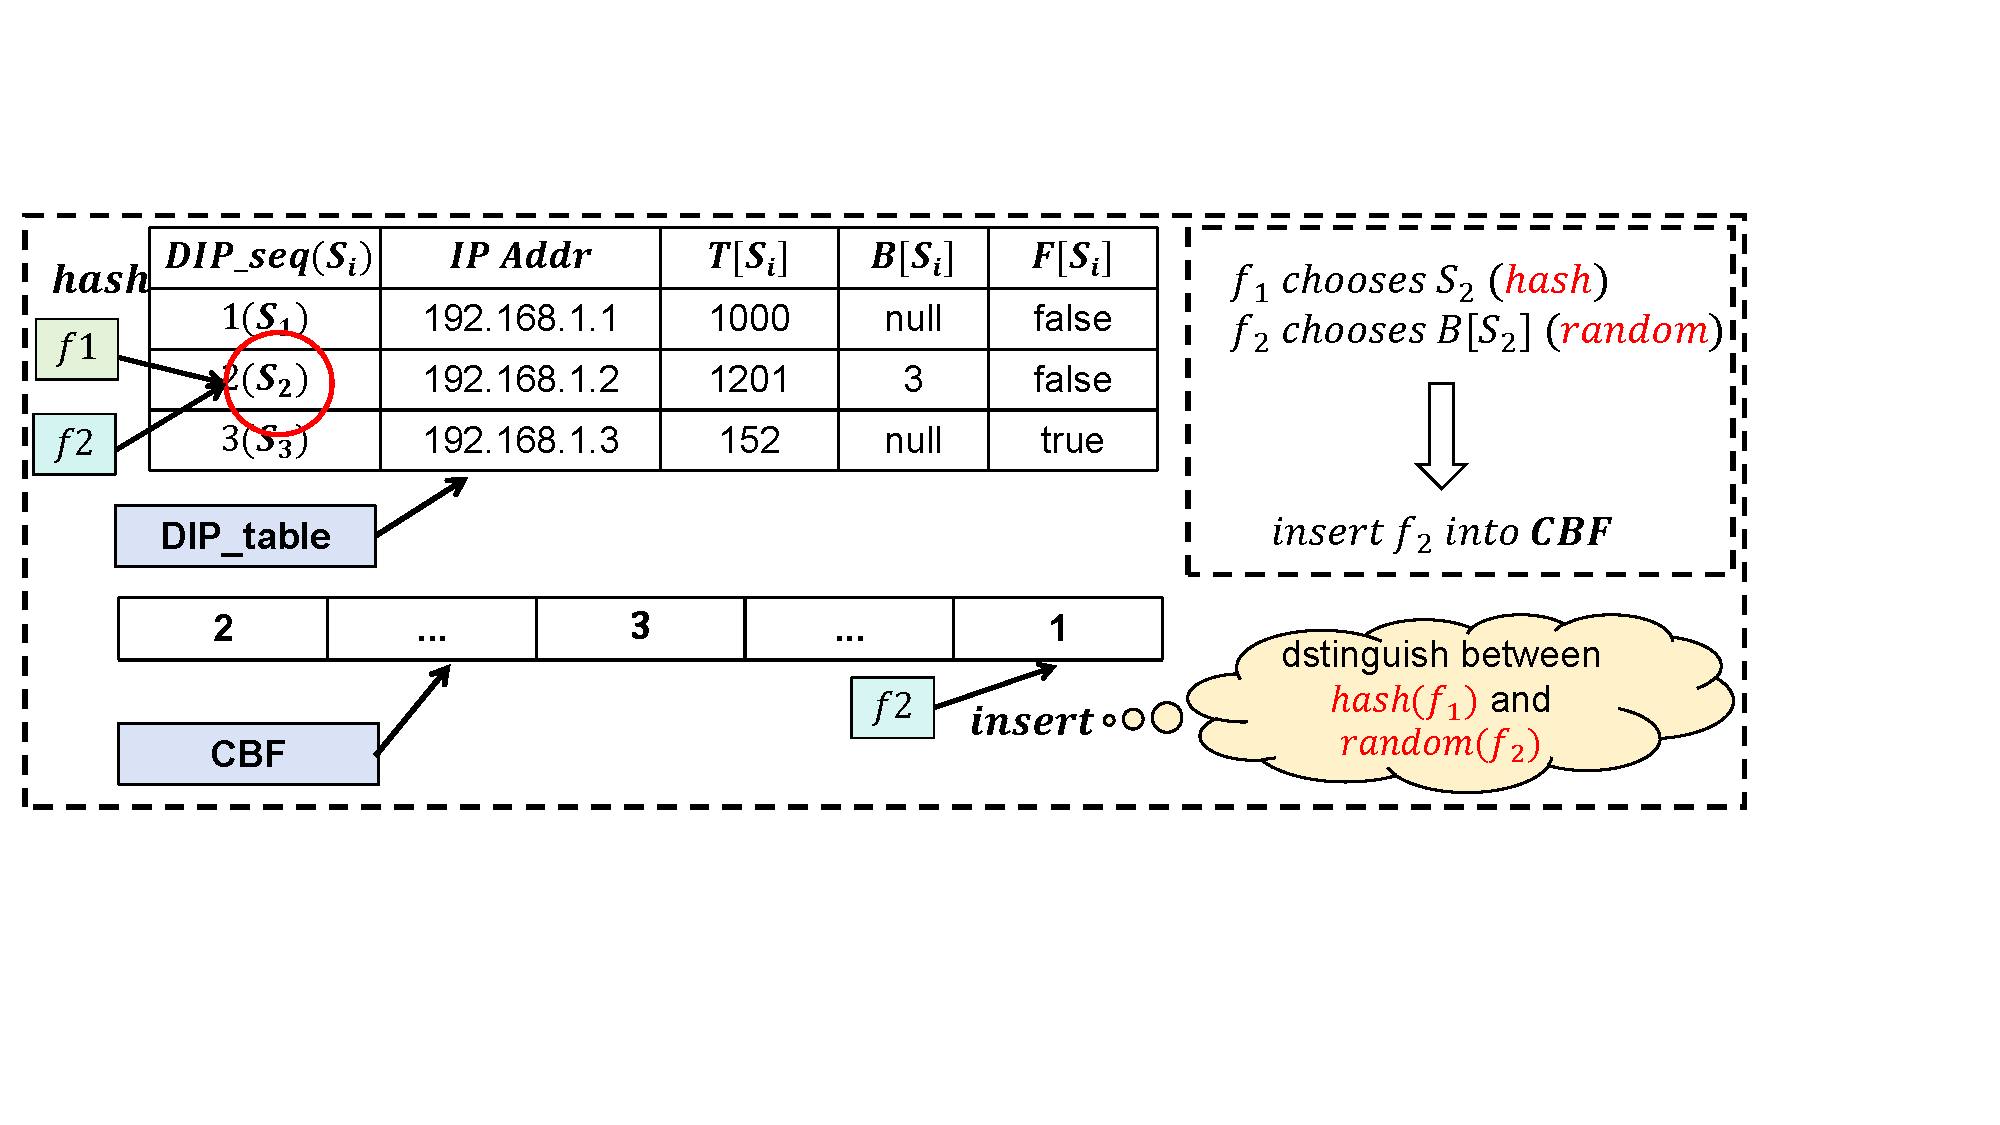
\includegraphics[width=1\linewidth]{figure/keeppcc3.pdf}}
	\caption{An example of keep PCC ($\Delta = 1000 (packets)$).}
	\label{7}
\end{figure}  